\documentclass[twoside]{book}

% Packages required by doxygen
\usepackage{calc}
\usepackage{doxygen}
\usepackage{graphicx}
\usepackage[utf8]{inputenc}
\usepackage{makeidx}
\usepackage{multicol}
\usepackage{multirow}
\usepackage{textcomp}
\usepackage[table]{xcolor}

% Font selection
\usepackage[T1]{fontenc}
\usepackage{mathptmx}
\usepackage[scaled=.90]{helvet}
\usepackage{courier}
\usepackage{amssymb}
\usepackage{sectsty}
\renewcommand{\familydefault}{\sfdefault}
\allsectionsfont{%
  \fontseries{bc}\selectfont%
  \color{darkgray}%
}
\renewcommand{\DoxyLabelFont}{%
  \fontseries{bc}\selectfont%
  \color{darkgray}%
}

% Page & text layout
\usepackage{geometry}
\geometry{%
  a4paper,%
  top=2.5cm,%
  bottom=2.5cm,%
  left=2.5cm,%
  right=2.5cm%
}
\tolerance=750
\hfuzz=15pt
\hbadness=750
\setlength{\emergencystretch}{15pt}
\setlength{\parindent}{0cm}
\setlength{\parskip}{0.2cm}
\makeatletter
\renewcommand{\paragraph}{%
  \@startsection{paragraph}{4}{0ex}{-1.0ex}{1.0ex}{%
    \normalfont\normalsize\bfseries\SS@parafont%
  }%
}
\renewcommand{\subparagraph}{%
  \@startsection{subparagraph}{5}{0ex}{-1.0ex}{1.0ex}{%
    \normalfont\normalsize\bfseries\SS@subparafont%
  }%
}
\makeatother

% Headers & footers
\usepackage{fancyhdr}
\pagestyle{fancyplain}
\fancyhead[LE]{\fancyplain{}{\bfseries\thepage}}
\fancyhead[CE]{\fancyplain{}{}}
\fancyhead[RE]{\fancyplain{}{\bfseries\leftmark}}
\fancyhead[LO]{\fancyplain{}{\bfseries\rightmark}}
\fancyhead[CO]{\fancyplain{}{}}
\fancyhead[RO]{\fancyplain{}{\bfseries\thepage}}
\fancyfoot[LE]{\fancyplain{}{}}
\fancyfoot[CE]{\fancyplain{}{}}
\fancyfoot[RE]{\fancyplain{}{\bfseries\scriptsize Generated on Fri Dec 6 2013 16\-:42\-:44 for Jeu Qt by Doxygen }}
\fancyfoot[LO]{\fancyplain{}{\bfseries\scriptsize Generated on Fri Dec 6 2013 16\-:42\-:44 for Jeu Qt by Doxygen }}
\fancyfoot[CO]{\fancyplain{}{}}
\fancyfoot[RO]{\fancyplain{}{}}
\renewcommand{\footrulewidth}{0.4pt}
\renewcommand{\chaptermark}[1]{%
  \markboth{#1}{}%
}
\renewcommand{\sectionmark}[1]{%
  \markright{\thesection\ #1}%
}

% Indices & bibliography
\usepackage{natbib}
\usepackage[titles]{tocloft}
\setcounter{tocdepth}{3}
\setcounter{secnumdepth}{5}
\makeindex

% Hyperlinks (required, but should be loaded last)
\usepackage{ifpdf}
\ifpdf
  \usepackage[pdftex,pagebackref=true]{hyperref}
\else
  \usepackage[ps2pdf,pagebackref=true]{hyperref}
\fi
\hypersetup{%
  colorlinks=true,%
  linkcolor=blue,%
  citecolor=blue,%
  unicode%
}

% Custom commands
\newcommand{\clearemptydoublepage}{%
  \newpage{\pagestyle{empty}\cleardoublepage}%
}


%===== C O N T E N T S =====

\begin{document}

% Titlepage & ToC
\hypersetup{pageanchor=false}
\pagenumbering{roman}
\begin{titlepage}
\vspace*{7cm}
\begin{center}%
{\Large Jeu Qt \\[1ex]\large 0.\-9 }\\
\vspace*{1cm}
{\large Generated by Doxygen 1.8.5}\\
\vspace*{0.5cm}
{\small Fri Dec 6 2013 16:42:44}\\
\end{center}
\end{titlepage}
\clearemptydoublepage
\tableofcontents
\clearemptydoublepage
\pagenumbering{arabic}
\hypersetup{pageanchor=true}

%--- Begin generated contents ---
\chapter{Jeu\-Qt}
\label{md__r_e_a_d_m_e}
\hypertarget{md__r_e_a_d_m_e}{}
Jeu \-: Joueur 1

Chaque joueur dispose de trois pions qu'ils peuvent poser un par un sur une surface de 3x3 chacun leur tour. Une fois les trois pions placés, un pion peut être déplacé, d'un point à un autre. Un emplacement ne peut être occupé que par un seul pion. La partie se termine une fois les trois pions alignés sur une même ligne, colonne ou diagonale. 
\chapter{Namespace Index}
\section{Namespace List}
Here is a list of all documented namespaces with brief descriptions\-:\begin{DoxyCompactList}
\item\contentsline{section}{\hyperlink{namespace_ui}{Ui} }{\pageref{namespace_ui}}{}
\end{DoxyCompactList}

\chapter{Hierarchical Index}
\section{Class Hierarchy}
This inheritance list is sorted roughly, but not completely, alphabetically\-:\begin{DoxyCompactList}
\item Q\-Label\begin{DoxyCompactList}
\item \contentsline{section}{emplacement}{\pageref{classemplacement}}{}
\item \contentsline{section}{joueur}{\pageref{classjoueur}}{}
\end{DoxyCompactList}
\item Q\-Main\-Window\begin{DoxyCompactList}
\item \contentsline{section}{Main\-Window}{\pageref{class_main_window}}{}
\end{DoxyCompactList}
\item \contentsline{section}{Ui\-\_\-\-Main\-Window}{\pageref{class_ui___main_window}}{}
\begin{DoxyCompactList}
\item \contentsline{section}{Ui\-:\-:Main\-Window}{\pageref{class_ui_1_1_main_window}}{}
\end{DoxyCompactList}
\end{DoxyCompactList}

\chapter{Class Index}
\section{Class List}
Here are the classes, structs, unions and interfaces with brief descriptions\-:\begin{DoxyCompactList}
\item\contentsline{section}{\hyperlink{classemplacement}{emplacement} }{\pageref{classemplacement}}{}
\item\contentsline{section}{\hyperlink{classjoueur}{joueur} }{\pageref{classjoueur}}{}
\item\contentsline{section}{\hyperlink{class_ui_1_1_main_window}{Ui\-::\-Main\-Window} }{\pageref{class_ui_1_1_main_window}}{}
\item\contentsline{section}{\hyperlink{class_main_window}{Main\-Window} \\*Classe \hyperlink{class_main_window}{Main\-Window} \-: public Q\-Main\-Window }{\pageref{class_main_window}}{}
\item\contentsline{section}{\hyperlink{class_ui___main_window}{Ui\-\_\-\-Main\-Window} }{\pageref{class_ui___main_window}}{}
\end{DoxyCompactList}

\chapter{Namespace Documentation}
\hypertarget{namespace_ui}{\section{Ui Namespace Reference}
\label{namespace_ui}\index{Ui@{Ui}}
}
\subsection*{Classes}
\begin{DoxyCompactItemize}
\item 
class \hyperlink{class_ui_1_1_main_window}{Main\-Window}
\end{DoxyCompactItemize}


\subsection{Detailed Description}

\begin{DoxyCodeInclude}
\end{DoxyCodeInclude}
 \hyperlink{emplacement_8h_source}{emplacement.\-h} 
\chapter{Class Documentation}
\hypertarget{classemplacement}{\section{emplacement Class Reference}
\label{classemplacement}\index{emplacement@{emplacement}}
}


Classe emplacement \-: public Q\-Label.  




{\ttfamily \#include $<$emplacement.\-h$>$}

Inheritance diagram for emplacement\-:\begin{figure}[H]
\begin{center}
\leavevmode
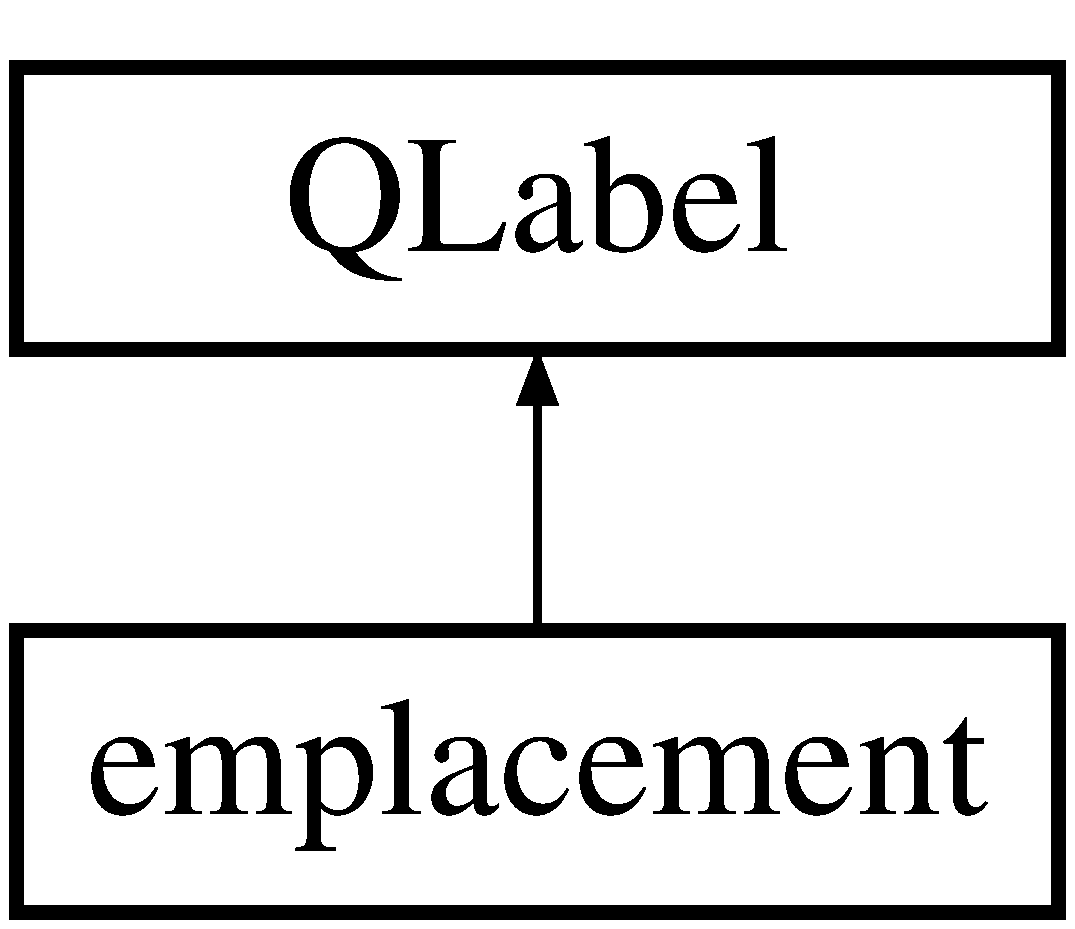
\includegraphics[height=2.000000cm]{classemplacement}
\end{center}
\end{figure}
\subsection*{Public Slots}
\begin{DoxyCompactItemize}
\item 
\hypertarget{classemplacement_afd15b612d02b7cbfd0480b5b380c2b07}{bool \hyperlink{classemplacement_afd15b612d02b7cbfd0480b5b380c2b07}{est\-Vide} ()}\label{classemplacement_afd15b612d02b7cbfd0480b5b380c2b07}

\begin{DoxyCompactList}\small\item\em Si l'emplacement est vide de pion. \end{DoxyCompactList}\item 
\hypertarget{classemplacement_a70e22f75b934e4daa40582708c4e01f5}{bool \hyperlink{classemplacement_a70e22f75b934e4daa40582708c4e01f5}{jouxte} (\hyperlink{classemplacement}{emplacement} $\ast$e)}\label{classemplacement_a70e22f75b934e4daa40582708c4e01f5}

\begin{DoxyCompactList}\small\item\em Si l'emplacement est jouxte à celui actuel. \end{DoxyCompactList}\item 
\hypertarget{classemplacement_a9e57590839f9c185d962030b221b8ea1}{void \hyperlink{classemplacement_a9e57590839f9c185d962030b221b8ea1}{set\-Joueur} (\hyperlink{classjoueur}{joueur} $\ast$)}\label{classemplacement_a9e57590839f9c185d962030b221b8ea1}

\begin{DoxyCompactList}\small\item\em Set un joueur. \end{DoxyCompactList}\item 
\hypertarget{classemplacement_ada71fd6bec4969e4ef5be1a610d712a4}{void \hyperlink{classemplacement_ada71fd6bec4969e4ef5be1a610d712a4}{vider} ()}\label{classemplacement_ada71fd6bec4969e4ef5be1a610d712a4}

\begin{DoxyCompactList}\small\item\em Vide l'emplacement. \end{DoxyCompactList}\item 
\hypertarget{classemplacement_aae4d4694984d645ddb397b5847032fa0}{void \hyperlink{classemplacement_aae4d4694984d645ddb397b5847032fa0}{jeu\-Adverse} ()}\label{classemplacement_aae4d4694984d645ddb397b5847032fa0}

\begin{DoxyCompactList}\small\item\em Tour du joueur adverse (réseau uniquement) \end{DoxyCompactList}\item 
\hypertarget{classemplacement_aa786f80d5617b15318e898f2ceacbe97}{void \hyperlink{classemplacement_aa786f80d5617b15318e898f2ceacbe97}{jeu\-Adverse\-Move} ()}\label{classemplacement_aa786f80d5617b15318e898f2ceacbe97}

\begin{DoxyCompactList}\small\item\em Tour du joueur adverse sans jeton (réseau uniquement) \end{DoxyCompactList}\end{DoxyCompactItemize}
\subsection*{Public Member Functions}
\begin{DoxyCompactItemize}
\item 
\hypertarget{classemplacement_ad52a33b25cbb300d91e13906db2a7cc3}{{\bfseries emplacement} (\hyperlink{class_main_window}{Main\-Window} $\ast$mum, Q\-Widget $\ast$parent=0)}\label{classemplacement_ad52a33b25cbb300d91e13906db2a7cc3}

\end{DoxyCompactItemize}
\subsection*{Public Attributes}
\begin{DoxyCompactItemize}
\item 
\hypertarget{classemplacement_aa0e8e131a1d8325f2245c56f8d2e6e8c}{int \hyperlink{classemplacement_aa0e8e131a1d8325f2245c56f8d2e6e8c}{ligne}}\label{classemplacement_aa0e8e131a1d8325f2245c56f8d2e6e8c}

\begin{DoxyCompactList}\small\item\em Ligne du plateau. \end{DoxyCompactList}\item 
\hypertarget{classemplacement_ac0af10e9e8d40e815a8b9633019406b1}{int \hyperlink{classemplacement_ac0af10e9e8d40e815a8b9633019406b1}{col}}\label{classemplacement_ac0af10e9e8d40e815a8b9633019406b1}

\begin{DoxyCompactList}\small\item\em Colonne du plateau. \end{DoxyCompactList}\item 
\hypertarget{classemplacement_ae496fbda5429d0d37f38c2c45f6b88b6}{\hyperlink{classjoueur}{joueur} $\ast$ \hyperlink{classemplacement_ae496fbda5429d0d37f38c2c45f6b88b6}{le\-Joueur}}\label{classemplacement_ae496fbda5429d0d37f38c2c45f6b88b6}

\begin{DoxyCompactList}\small\item\em Joueur. \end{DoxyCompactList}\end{DoxyCompactItemize}


\subsection{Detailed Description}
Classe emplacement \-: public Q\-Label. 

\begin{DoxyAuthor}{Author}
Alberto Hugo 
\end{DoxyAuthor}
\begin{DoxyVersion}{Version}
0.\-9 
\end{DoxyVersion}
\begin{DoxyDate}{Date}
2013-\/2014 
\end{DoxyDate}
\begin{DoxyPrecond}{Precondition}
Initialise la classe emplacement 
\end{DoxyPrecond}
\begin{DoxyCopyright}{Copyright}
G\-N\-U Public License. 
\end{DoxyCopyright}


The documentation for this class was generated from the following files\-:\begin{DoxyCompactItemize}
\item 
emplacement.\-h\item 
emplacement.\-cpp\end{DoxyCompactItemize}

\hypertarget{classjoueur}{\section{joueur Class Reference}
\label{classjoueur}\index{joueur@{joueur}}
}


Classe joueur \-: public Q\-Label.  




{\ttfamily \#include $<$joueur.\-h$>$}

Inheritance diagram for joueur\-:\begin{figure}[H]
\begin{center}
\leavevmode
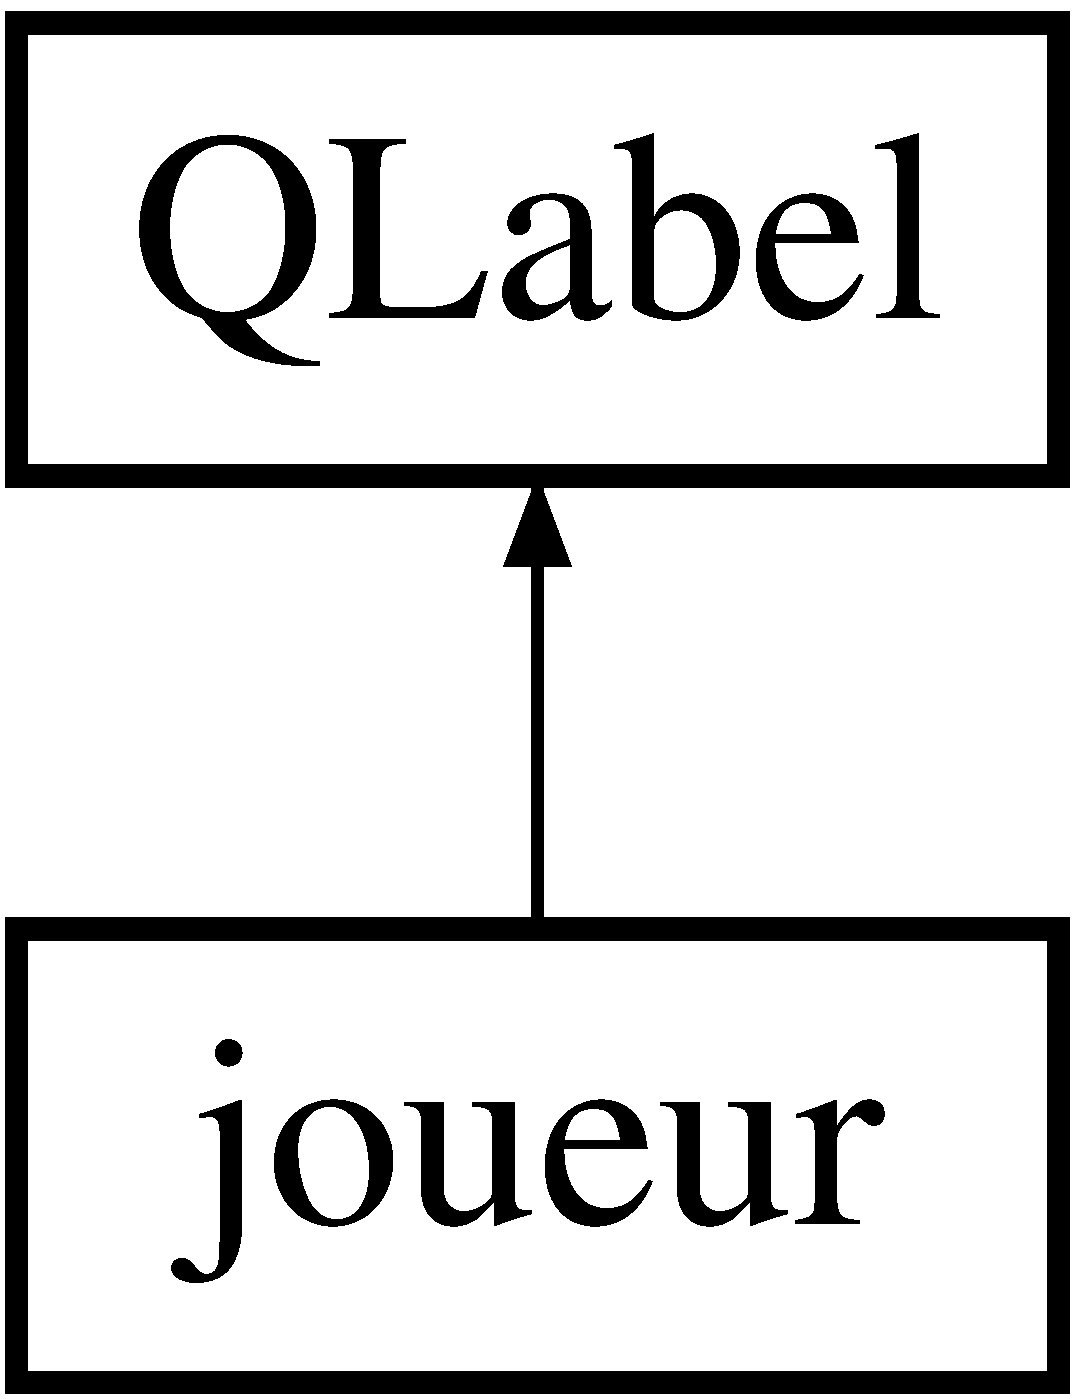
\includegraphics[height=2.000000cm]{classjoueur}
\end{center}
\end{figure}
\subsection*{Public Member Functions}
\begin{DoxyCompactItemize}
\item 
\hypertarget{classjoueur_a9f78a65e07011114967ef5c813a868cb}{{\bfseries joueur} (Q\-String l, Q\-String string\-Couleur, Q\-Widget $\ast$parent=0)}\label{classjoueur_a9f78a65e07011114967ef5c813a868cb}

\item 
\hypertarget{classjoueur_a6095d00e5c84a98694ae3f2ebbef48d8}{void \hyperlink{classjoueur_a6095d00e5c84a98694ae3f2ebbef48d8}{set\-Lettre} (Q\-String)}\label{classjoueur_a6095d00e5c84a98694ae3f2ebbef48d8}

\begin{DoxyCompactList}\small\item\em Met une lettre dans un Q\-String. \end{DoxyCompactList}\item 
\hypertarget{classjoueur_a7a91ed8fa89ad62545bae8e805565c39}{Q\-String \hyperlink{classjoueur_a7a91ed8fa89ad62545bae8e805565c39}{get\-Lettre} ()}\label{classjoueur_a7a91ed8fa89ad62545bae8e805565c39}

\begin{DoxyCompactList}\small\item\em Récupère la lettre du joueur. \end{DoxyCompactList}\item 
\hypertarget{classjoueur_a19403939c10d9a70b6035024978ca230}{Q\-Cursor $\ast$ \hyperlink{classjoueur_a19403939c10d9a70b6035024978ca230}{get\-Son\-Curseur} (Q\-String lequel)}\label{classjoueur_a19403939c10d9a70b6035024978ca230}

\begin{DoxyCompactList}\small\item\em Récupère le curseur du joueur actif. \end{DoxyCompactList}\item 
int \hyperlink{classjoueur_a80aefa29f51995d731605b5230840ac3}{get\-Nb\-Jeton} ()
\begin{DoxyCompactList}\small\item\em Récupère le nombre de jetons. \end{DoxyCompactList}\item 
void \hyperlink{classjoueur_a15c0ea5487cf6800e373cb1b1ed52b12}{reset\-Jeton} ()
\begin{DoxyCompactList}\small\item\em Initialise les jetons du joueur. \end{DoxyCompactList}\item 
\hypertarget{classjoueur_a1a1b8731c7eec4f854a65d83c3f6fc70}{void \hyperlink{classjoueur_a1a1b8731c7eec4f854a65d83c3f6fc70}{diminue\-Nb\-Jeton} ()}\label{classjoueur_a1a1b8731c7eec4f854a65d83c3f6fc70}

\begin{DoxyCompactList}\small\item\em Diminue le nombre de jeton par 1. \end{DoxyCompactList}\item 
Q\-String \hyperlink{classjoueur_a2992fc3e5e7f08794c001db796f5e925}{get\-Couleur} ()
\begin{DoxyCompactList}\small\item\em Récupère la couleur d'un joueur. \end{DoxyCompactList}\end{DoxyCompactItemize}


\subsection{Detailed Description}
Classe joueur \-: public Q\-Label. 

\begin{DoxyAuthor}{Author}
Alberto Hugo 
\end{DoxyAuthor}
\begin{DoxyVersion}{Version}
0.\-9 
\end{DoxyVersion}
\begin{DoxyDate}{Date}
2013-\/2014 
\end{DoxyDate}
\begin{DoxyPrecond}{Precondition}
Initialise la classe joueur 
\end{DoxyPrecond}
\begin{DoxyCopyright}{Copyright}
G\-N\-U Public License. 
\end{DoxyCopyright}


\subsection{Member Function Documentation}
\hypertarget{classjoueur_a2992fc3e5e7f08794c001db796f5e925}{\index{joueur@{joueur}!get\-Couleur@{get\-Couleur}}
\index{get\-Couleur@{get\-Couleur}!joueur@{joueur}}
\subsubsection[{get\-Couleur}]{\setlength{\rightskip}{0pt plus 5cm}Q\-String joueur\-::get\-Couleur (
\begin{DoxyParamCaption}
{}
\end{DoxyParamCaption}
)\hspace{0.3cm}{\ttfamily [inline]}}}\label{classjoueur_a2992fc3e5e7f08794c001db796f5e925}


Récupère la couleur d'un joueur. 

\begin{DoxyReturn}{Returns}
couleur 
\end{DoxyReturn}
\hypertarget{classjoueur_a80aefa29f51995d731605b5230840ac3}{\index{joueur@{joueur}!get\-Nb\-Jeton@{get\-Nb\-Jeton}}
\index{get\-Nb\-Jeton@{get\-Nb\-Jeton}!joueur@{joueur}}
\subsubsection[{get\-Nb\-Jeton}]{\setlength{\rightskip}{0pt plus 5cm}int joueur\-::get\-Nb\-Jeton (
\begin{DoxyParamCaption}
{}
\end{DoxyParamCaption}
)\hspace{0.3cm}{\ttfamily [inline]}}}\label{classjoueur_a80aefa29f51995d731605b5230840ac3}


Récupère le nombre de jetons. 

\begin{DoxyReturn}{Returns}
nombre de jeton 
\end{DoxyReturn}
\hypertarget{classjoueur_a15c0ea5487cf6800e373cb1b1ed52b12}{\index{joueur@{joueur}!reset\-Jeton@{reset\-Jeton}}
\index{reset\-Jeton@{reset\-Jeton}!joueur@{joueur}}
\subsubsection[{reset\-Jeton}]{\setlength{\rightskip}{0pt plus 5cm}void joueur\-::reset\-Jeton (
\begin{DoxyParamCaption}
{}
\end{DoxyParamCaption}
)\hspace{0.3cm}{\ttfamily [inline]}}}\label{classjoueur_a15c0ea5487cf6800e373cb1b1ed52b12}


Initialise les jetons du joueur. 

\begin{DoxyReturn}{Returns}
Le nombre de jeton reçoit 3 
\end{DoxyReturn}


The documentation for this class was generated from the following files\-:\begin{DoxyCompactItemize}
\item 
joueur.\-h\item 
joueur.\-cpp\end{DoxyCompactItemize}

\hypertarget{class_ui_1_1_main_window}{\section{Ui\-:\-:Main\-Window Class Reference}
\label{class_ui_1_1_main_window}\index{Ui\-::\-Main\-Window@{Ui\-::\-Main\-Window}}
}
Inheritance diagram for Ui\-:\-:Main\-Window\-:\begin{figure}[H]
\begin{center}
\leavevmode
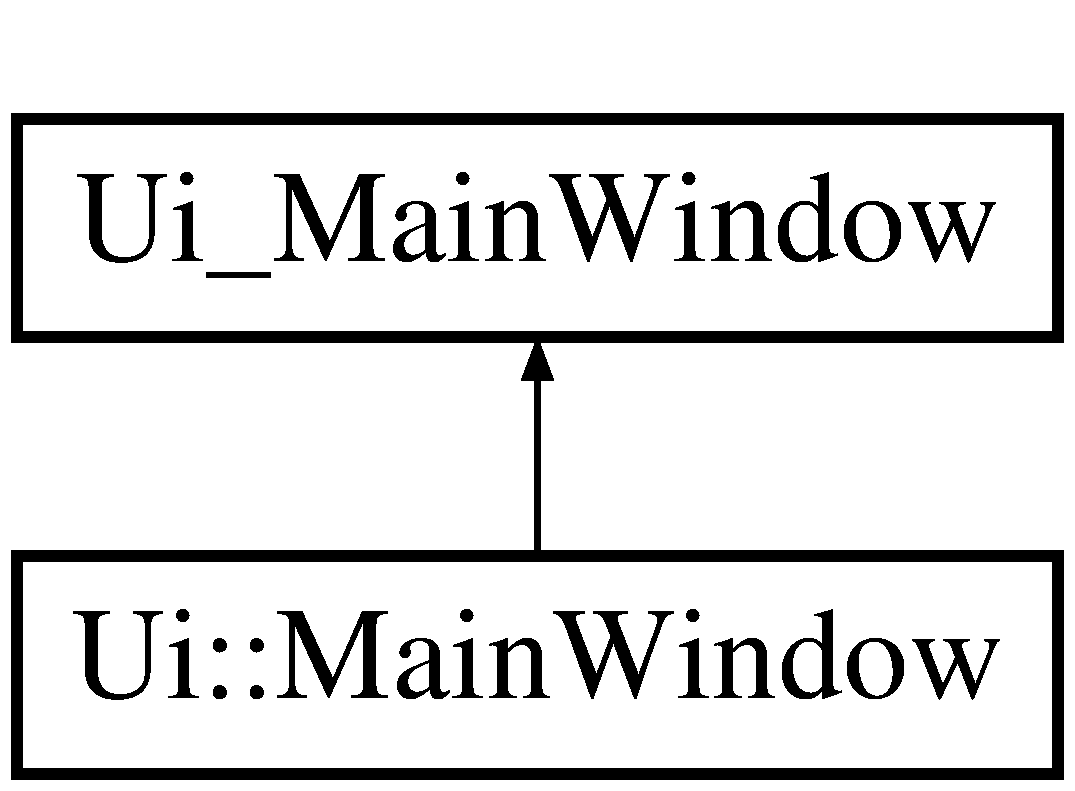
\includegraphics[height=2.000000cm]{class_ui_1_1_main_window}
\end{center}
\end{figure}
\subsection*{Additional Inherited Members}


The documentation for this class was generated from the following file\-:\begin{DoxyCompactItemize}
\item 
ui\-\_\-mainwindow.\-h\end{DoxyCompactItemize}

\hypertarget{class_main_window}{\section{Main\-Window Class Reference}
\label{class_main_window}\index{Main\-Window@{Main\-Window}}
}


Classe \hyperlink{class_main_window}{Main\-Window} \-: public Q\-Main\-Window.  




{\ttfamily \#include $<$mainwindow.\-h$>$}

Inheritance diagram for Main\-Window\-:\begin{figure}[H]
\begin{center}
\leavevmode
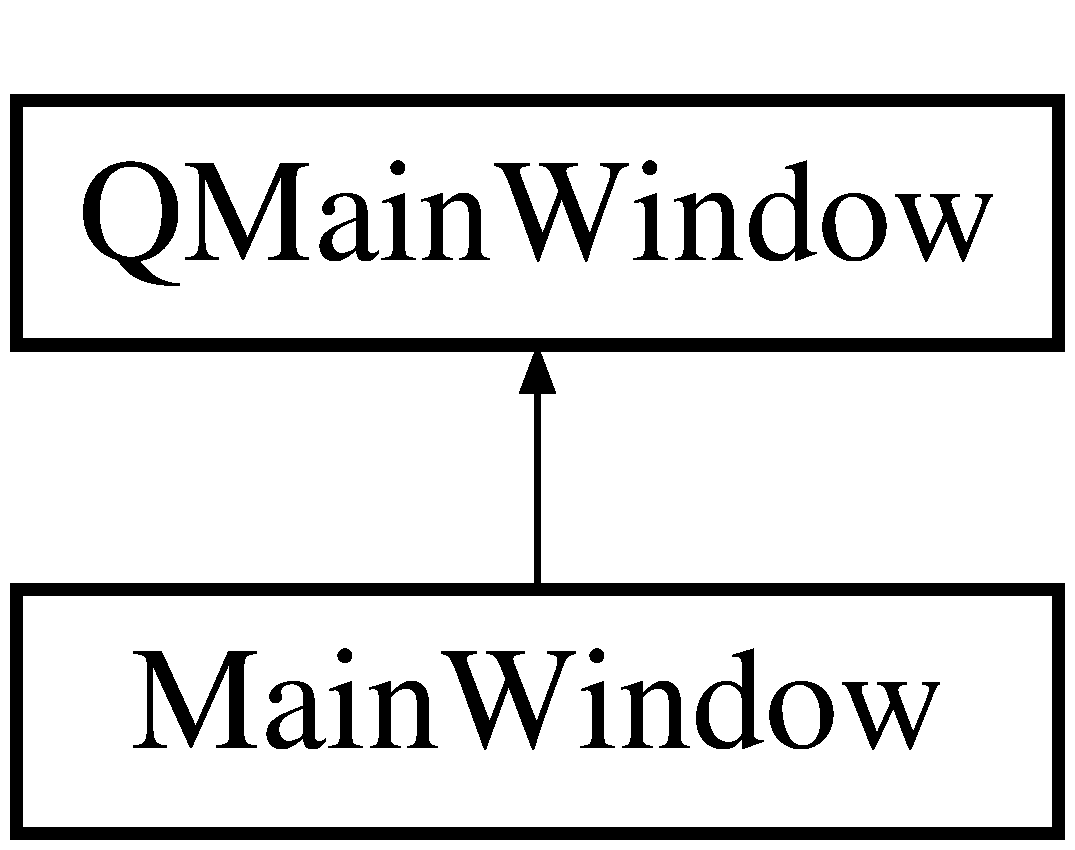
\includegraphics[height=2.000000cm]{class_main_window}
\end{center}
\end{figure}
\subsection*{Public Slots}
\begin{DoxyCompactItemize}
\item 
\hypertarget{class_main_window_a4ae4ac96dbfdcb80facbf7da0ae3fb5e}{bool \hyperlink{class_main_window_a4ae4ac96dbfdcb80facbf7da0ae3fb5e}{est\-Coince} (\hyperlink{classemplacement}{emplacement} $\ast$)}\label{class_main_window_a4ae4ac96dbfdcb80facbf7da0ae3fb5e}

\begin{DoxyCompactList}\small\item\em Si le pion est coincé et ne peut être déplcacé \end{DoxyCompactList}\item 
bool \hyperlink{class_main_window_ac3a2c00ad936408dce78d15697eeef24}{accessible} (\hyperlink{classemplacement}{emplacement} $\ast$e1, \hyperlink{classemplacement}{emplacement} $\ast$e2)
\begin{DoxyCompactList}\small\item\em Si l'emplacement est accéssible par le pion. \end{DoxyCompactList}\item 
void \hyperlink{class_main_window_a8e9fb499b85eef1d31b4caedcdad3424}{set\-Curseur} (Q\-Cursor \&cuseur)
\item 
void \hyperlink{class_main_window_aa423b534c9d408e59a52f6e7644ccdcb}{commence\-Partie} ()
\item 
void \hyperlink{class_main_window_acb2efdb6b0b137cf2e44d6bd2fbb3aec}{reception\-Donnees} ()
\begin{DoxyCompactList}\small\item\em Réception des données. \end{DoxyCompactList}\item 
\hypertarget{class_main_window_a52d0b54e86461bd0f4738921651c15a2}{void \hyperlink{class_main_window_a52d0b54e86461bd0f4738921651c15a2}{changement\-Etat\-Socket} (Q\-Abstract\-Socket\-::\-Socket\-State etat)}\label{class_main_window_a52d0b54e86461bd0f4738921651c15a2}

\begin{DoxyCompactList}\small\item\em Fonctionnalité à développer. \end{DoxyCompactList}\end{DoxyCompactItemize}
\subsection*{Public Member Functions}
\begin{DoxyCompactItemize}
\item 
\hyperlink{class_main_window_a8b244be8b7b7db1b08de2a2acb9409db}{Main\-Window} (Q\-Widget $\ast$parent=0)
\begin{DoxyCompactList}\small\item\em Le constructeur. \end{DoxyCompactList}\item 
\hyperlink{class_main_window_ae98d00a93bc118200eeef9f9bba1dba7}{$\sim$\-Main\-Window} ()
\begin{DoxyCompactList}\small\item\em Le destructeur. \end{DoxyCompactList}\item 
\hypertarget{class_main_window_a1eefa05031d74694e4249a8c68741122}{void {\bfseries set\-Emplacement\-Deplace} (\hyperlink{classemplacement}{emplacement} $\ast$e)}\label{class_main_window_a1eefa05031d74694e4249a8c68741122}

\item 
\hypertarget{class_main_window_a3ab75adb0221eb5e362f2070f71ebc22}{void \hyperlink{class_main_window_a3ab75adb0221eb5e362f2070f71ebc22}{reset\-Curseur} ()}\label{class_main_window_a3ab75adb0221eb5e362f2070f71ebc22}

\begin{DoxyCompactList}\small\item\em Remise du curseur d'origine. \end{DoxyCompactList}\item 
\hypertarget{class_main_window_a3c0bedf7eae76f0c5ca35bd16491b919}{void \hyperlink{class_main_window_a3c0bedf7eae76f0c5ca35bd16491b919}{changement} ()}\label{class_main_window_a3c0bedf7eae76f0c5ca35bd16491b919}

\begin{DoxyCompactList}\small\item\em Changement du joueur en cours. \end{DoxyCompactList}\item 
bool \hyperlink{class_main_window_a6dc1f84d9bc6e8ab7f1bb6bc04e2db49}{ligne} (int no)
\begin{DoxyCompactList}\small\item\em Ligne du plateau de jeu (numéro de la ligne) \end{DoxyCompactList}\item 
bool \hyperlink{class_main_window_a85653198b42750c0f09876f0af3715d7}{col} (int no)
\begin{DoxyCompactList}\small\item\em Colonne du plateau de jeu (numéro de la colonne) \end{DoxyCompactList}\item 
bool \hyperlink{class_main_window_a7b80bba7c56fbcc016dbc004d208ec31}{diag} (int no)
\begin{DoxyCompactList}\small\item\em Diagonale du plateau de jeu (numéro de la diagonale) \end{DoxyCompactList}\item 
bool \hyperlink{class_main_window_a1810f8a7d5a8497d738d909efca8947b}{deja\-Gagne} (\hyperlink{classjoueur}{joueur} $\ast$un\-Joueur)
\begin{DoxyCompactList}\small\item\em Si le joueur à déjà gagné (le joueur) \end{DoxyCompactList}\end{DoxyCompactItemize}
\subsection*{Public Attributes}
\begin{DoxyCompactItemize}
\item 
\hyperlink{classjoueur}{joueur} $\ast$ \hyperlink{class_main_window_a70a2607d9b49f3b5cd32afec1cb614a9}{joueur\-Actif}
\begin{DoxyCompactList}\small\item\em Le joueur qui est entrain de jouer. \end{DoxyCompactList}\item 
\hyperlink{classjoueur}{joueur} $\ast$ \hyperlink{class_main_window_ac8503f9eb4259016c7858e59aa31c1a4}{joueur\-Humain}
\item 
\hyperlink{classjoueur}{joueur} $\ast$ \hyperlink{class_main_window_acb5c1aad1ac317404027da04e4a175d3}{joueur\-Ordi}
\item 
\hypertarget{class_main_window_aa201a7ead9510f42427bd7b28e690df1}{\hyperlink{classemplacement}{emplacement} $\ast$ \hyperlink{class_main_window_aa201a7ead9510f42427bd7b28e690df1}{emplacement\-Deplace}}\label{class_main_window_aa201a7ead9510f42427bd7b28e690df1}

\begin{DoxyCompactList}\small\item\em Le pion déplacé \end{DoxyCompactList}\item 
\hypertarget{class_main_window_a40ca81795033b7d295527bc860f716cf}{Q\-Pixmap \hyperlink{class_main_window_a40ca81795033b7d295527bc860f716cf}{pixmap\-Empty\-Emplacement}}\label{class_main_window_a40ca81795033b7d295527bc860f716cf}

\begin{DoxyCompactList}\small\item\em L'image du pion vide. \end{DoxyCompactList}\item 
\hypertarget{class_main_window_abe41e7eada364f38acf9bfe58cc6eee3}{Q\-Timer $\ast$ \hyperlink{class_main_window_abe41e7eada364f38acf9bfe58cc6eee3}{timer\-Tour}}\label{class_main_window_abe41e7eada364f38acf9bfe58cc6eee3}

\begin{DoxyCompactList}\small\item\em Le temps pour chaque tour (sablier). \end{DoxyCompactList}\item 
bool \hyperlink{class_main_window_a00d26707b5d27cc6ce07479a46244692}{partie\-Terminee}
\begin{DoxyCompactList}\small\item\em Si la partie est déjà terminée. \end{DoxyCompactList}\item 
bool \hyperlink{class_main_window_ac4fe06d6d85536567fd86733f8cdf6c9}{serveur}
\begin{DoxyCompactList}\small\item\em Si l'application est un serveur. \end{DoxyCompactList}\item 
bool \hyperlink{class_main_window_a8037ff2bca42ebb5858b0cebd5ef9bb7}{jvj}
\begin{DoxyCompactList}\small\item\em Si l'application est un joueur contre un joueur. \end{DoxyCompactList}\item 
bool \hyperlink{class_main_window_a68723ed09b653ede2bd97dd85928076b}{ia\-On}
\begin{DoxyCompactList}\small\item\em Si l'application est contre un ordinateur. \end{DoxyCompactList}\item 
\hypertarget{class_main_window_a4b1e890b4b33f6ff8c22621d2ce55c2d}{Q\-Tcp\-Server $\ast$ \hyperlink{class_main_window_a4b1e890b4b33f6ff8c22621d2ce55c2d}{server}}\label{class_main_window_a4b1e890b4b33f6ff8c22621d2ce55c2d}

\begin{DoxyCompactList}\small\item\em Socket serveur. \end{DoxyCompactList}\item 
\hypertarget{class_main_window_af1832d65e85d46eb6cd8492cbec60864}{Q\-Tcp\-Socket $\ast$ \hyperlink{class_main_window_af1832d65e85d46eb6cd8492cbec60864}{la\-Socket}}\label{class_main_window_af1832d65e85d46eb6cd8492cbec60864}

\begin{DoxyCompactList}\small\item\em Socket client. \end{DoxyCompactList}\end{DoxyCompactItemize}


\subsection{Detailed Description}
Classe \hyperlink{class_main_window}{Main\-Window} \-: public Q\-Main\-Window. 

\begin{DoxyAuthor}{Author}
Alberto Hugo 
\end{DoxyAuthor}
\begin{DoxyVersion}{Version}
0.\-9 
\end{DoxyVersion}
\begin{DoxyDate}{Date}
2013-\/2014 
\end{DoxyDate}
\begin{DoxyPrecond}{Precondition}
Initialise l'application 
\end{DoxyPrecond}
\begin{DoxyCopyright}{Copyright}
G\-N\-U Public License. 
\end{DoxyCopyright}


\subsection{Constructor \& Destructor Documentation}
\hypertarget{class_main_window_a8b244be8b7b7db1b08de2a2acb9409db}{\index{Main\-Window@{Main\-Window}!Main\-Window@{Main\-Window}}
\index{Main\-Window@{Main\-Window}!MainWindow@{Main\-Window}}
\subsubsection[{Main\-Window}]{\setlength{\rightskip}{0pt plus 5cm}Main\-Window\-::\-Main\-Window (
\begin{DoxyParamCaption}
\item[{Q\-Widget $\ast$}]{parent = {\ttfamily 0}}
\end{DoxyParamCaption}
)\hspace{0.3cm}{\ttfamily [explicit]}}}\label{class_main_window_a8b244be8b7b7db1b08de2a2acb9409db}


Le constructeur. 

\hyperlink{class_main_window}{Main\-Window} 
\begin{DoxyParams}{Parameters}
{\em parent,Met} & le codec U\-T\-F-\/8 en place, Construit l'interface, Met en place le socket, Crée le plateau de jeu, Connect le timer, Initialise la partie \\
\hline
\end{DoxyParams}
\hypertarget{class_main_window_ae98d00a93bc118200eeef9f9bba1dba7}{\index{Main\-Window@{Main\-Window}!$\sim$\-Main\-Window@{$\sim$\-Main\-Window}}
\index{$\sim$\-Main\-Window@{$\sim$\-Main\-Window}!MainWindow@{Main\-Window}}
\subsubsection[{$\sim$\-Main\-Window}]{\setlength{\rightskip}{0pt plus 5cm}Main\-Window\-::$\sim$\-Main\-Window (
\begin{DoxyParamCaption}
{}
\end{DoxyParamCaption}
)}}\label{class_main_window_ae98d00a93bc118200eeef9f9bba1dba7}


Le destructeur. 

Détruit la mémoire allouée par le programme 

\subsection{Member Function Documentation}
\hypertarget{class_main_window_ac3a2c00ad936408dce78d15697eeef24}{\index{Main\-Window@{Main\-Window}!accessible@{accessible}}
\index{accessible@{accessible}!MainWindow@{Main\-Window}}
\subsubsection[{accessible}]{\setlength{\rightskip}{0pt plus 5cm}bool Main\-Window\-::accessible (
\begin{DoxyParamCaption}
\item[{{\bf emplacement} $\ast$}]{e1, }
\item[{{\bf emplacement} $\ast$}]{e2}
\end{DoxyParamCaption}
)\hspace{0.3cm}{\ttfamily [slot]}}}\label{class_main_window_ac3a2c00ad936408dce78d15697eeef24}


Si l'emplacement est accéssible par le pion. 

\begin{DoxyReturn}{Returns}
l'emplacement est vide, et il est jouxte au pion qui est entrain d'être joué 
\end{DoxyReturn}
\hypertarget{class_main_window_a85653198b42750c0f09876f0af3715d7}{\index{Main\-Window@{Main\-Window}!col@{col}}
\index{col@{col}!MainWindow@{Main\-Window}}
\subsubsection[{col}]{\setlength{\rightskip}{0pt plus 5cm}bool Main\-Window\-::col (
\begin{DoxyParamCaption}
\item[{int}]{no}
\end{DoxyParamCaption}
)}}\label{class_main_window_a85653198b42750c0f09876f0af3715d7}


Colonne du plateau de jeu (numéro de la colonne) 

Retourne true ou false en fonction de la colonne \begin{DoxyReturn}{Returns}
true si la colonne est pleine par un même joueur 

false si la colonne est vide ou pleine par plus d'un joueur 
\end{DoxyReturn}
\hypertarget{class_main_window_aa423b534c9d408e59a52f6e7644ccdcb}{\index{Main\-Window@{Main\-Window}!commence\-Partie@{commence\-Partie}}
\index{commence\-Partie@{commence\-Partie}!MainWindow@{Main\-Window}}
\subsubsection[{commence\-Partie}]{\setlength{\rightskip}{0pt plus 5cm}void Main\-Window\-::commence\-Partie (
\begin{DoxyParamCaption}
{}
\end{DoxyParamCaption}
)\hspace{0.3cm}{\ttfamily [slot]}}}\label{class_main_window_aa423b534c9d408e59a52f6e7644ccdcb}
Commence une partie en réseau quand un client à trouvé un serveur \hypertarget{class_main_window_a1810f8a7d5a8497d738d909efca8947b}{\index{Main\-Window@{Main\-Window}!deja\-Gagne@{deja\-Gagne}}
\index{deja\-Gagne@{deja\-Gagne}!MainWindow@{Main\-Window}}
\subsubsection[{deja\-Gagne}]{\setlength{\rightskip}{0pt plus 5cm}bool Main\-Window\-::deja\-Gagne (
\begin{DoxyParamCaption}
\item[{{\bf joueur} $\ast$}]{un\-Joueur}
\end{DoxyParamCaption}
)}}\label{class_main_window_a1810f8a7d5a8497d738d909efca8947b}


Si le joueur à déjà gagné (le joueur) 

\begin{DoxyReturn}{Returns}
true si la partie à déjà été gagné par un joueur 

false si la partie n'est pas encore gagné 
\end{DoxyReturn}
\hypertarget{class_main_window_a7b80bba7c56fbcc016dbc004d208ec31}{\index{Main\-Window@{Main\-Window}!diag@{diag}}
\index{diag@{diag}!MainWindow@{Main\-Window}}
\subsubsection[{diag}]{\setlength{\rightskip}{0pt plus 5cm}bool Main\-Window\-::diag (
\begin{DoxyParamCaption}
\item[{int}]{no}
\end{DoxyParamCaption}
)}}\label{class_main_window_a7b80bba7c56fbcc016dbc004d208ec31}


Diagonale du plateau de jeu (numéro de la diagonale) 

Retourne true ou false en fonction de la diagonale \begin{DoxyReturn}{Returns}
true si la diagonale est pleine par un même joueur 

false si la diagonaleest vide ou pleine par plus d'un joueur 
\end{DoxyReturn}
\hypertarget{class_main_window_a6dc1f84d9bc6e8ab7f1bb6bc04e2db49}{\index{Main\-Window@{Main\-Window}!ligne@{ligne}}
\index{ligne@{ligne}!MainWindow@{Main\-Window}}
\subsubsection[{ligne}]{\setlength{\rightskip}{0pt plus 5cm}bool Main\-Window\-::ligne (
\begin{DoxyParamCaption}
\item[{int}]{no}
\end{DoxyParamCaption}
)}}\label{class_main_window_a6dc1f84d9bc6e8ab7f1bb6bc04e2db49}


Ligne du plateau de jeu (numéro de la ligne) 

Retourne true ou false en fonction de la ligne \begin{DoxyReturn}{Returns}
true si la ligne est pleine par un même joueur 

false si la ligne est vide ou pleine par plus d'un joueur 
\end{DoxyReturn}
\hypertarget{class_main_window_acb2efdb6b0b137cf2e44d6bd2fbb3aec}{\index{Main\-Window@{Main\-Window}!reception\-Donnees@{reception\-Donnees}}
\index{reception\-Donnees@{reception\-Donnees}!MainWindow@{Main\-Window}}
\subsubsection[{reception\-Donnees}]{\setlength{\rightskip}{0pt plus 5cm}void Main\-Window\-::reception\-Donnees (
\begin{DoxyParamCaption}
{}
\end{DoxyParamCaption}
)\hspace{0.3cm}{\ttfamily [slot]}}}\label{class_main_window_acb2efdb6b0b137cf2e44d6bd2fbb3aec}


Réception des données. 

Échange des données entre le serveur et le client \hypertarget{class_main_window_a8e9fb499b85eef1d31b4caedcdad3424}{\index{Main\-Window@{Main\-Window}!set\-Curseur@{set\-Curseur}}
\index{set\-Curseur@{set\-Curseur}!MainWindow@{Main\-Window}}
\subsubsection[{set\-Curseur}]{\setlength{\rightskip}{0pt plus 5cm}void Main\-Window\-::set\-Curseur (
\begin{DoxyParamCaption}
\item[{Q\-Cursor \&}]{cuseur}
\end{DoxyParamCaption}
)\hspace{0.3cm}{\ttfamily [slot]}}}\label{class_main_window_a8e9fb499b85eef1d31b4caedcdad3424}
Modifie le curseur courant par le curseur qui va bien 

\subsection{Member Data Documentation}
\hypertarget{class_main_window_a68723ed09b653ede2bd97dd85928076b}{\index{Main\-Window@{Main\-Window}!ia\-On@{ia\-On}}
\index{ia\-On@{ia\-On}!MainWindow@{Main\-Window}}
\subsubsection[{ia\-On}]{\setlength{\rightskip}{0pt plus 5cm}bool Main\-Window\-::ia\-On}}\label{class_main_window_a68723ed09b653ede2bd97dd85928076b}


Si l'application est contre un ordinateur. 

\begin{DoxyReturn}{Returns}
true si l'application est contre un ordinateur 

false si l'application n'est pas contre un ordinateur 
\end{DoxyReturn}
\hypertarget{class_main_window_a70a2607d9b49f3b5cd32afec1cb614a9}{\index{Main\-Window@{Main\-Window}!joueur\-Actif@{joueur\-Actif}}
\index{joueur\-Actif@{joueur\-Actif}!MainWindow@{Main\-Window}}
\subsubsection[{joueur\-Actif}]{\setlength{\rightskip}{0pt plus 5cm}{\bf joueur}$\ast$ Main\-Window\-::joueur\-Actif}}\label{class_main_window_a70a2607d9b49f3b5cd32afec1cb614a9}


Le joueur qui est entrain de jouer. 

Comporte, soit le joueur humain (joueur 1), soit le joueur ordi (joueur 2) \begin{DoxyReturn}{Returns}
Le joueur courrant 
\end{DoxyReturn}
\hypertarget{class_main_window_ac8503f9eb4259016c7858e59aa31c1a4}{\index{Main\-Window@{Main\-Window}!joueur\-Humain@{joueur\-Humain}}
\index{joueur\-Humain@{joueur\-Humain}!MainWindow@{Main\-Window}}
\subsubsection[{joueur\-Humain}]{\setlength{\rightskip}{0pt plus 5cm}{\bf joueur}$\ast$ Main\-Window\-::joueur\-Humain}}\label{class_main_window_ac8503f9eb4259016c7858e59aa31c1a4}
Le joueur humain, et aussi le joueur 1 \begin{DoxyReturn}{Returns}
Le joueur 1 
\end{DoxyReturn}
\hypertarget{class_main_window_acb5c1aad1ac317404027da04e4a175d3}{\index{Main\-Window@{Main\-Window}!joueur\-Ordi@{joueur\-Ordi}}
\index{joueur\-Ordi@{joueur\-Ordi}!MainWindow@{Main\-Window}}
\subsubsection[{joueur\-Ordi}]{\setlength{\rightskip}{0pt plus 5cm}{\bf joueur}$\ast$ Main\-Window\-::joueur\-Ordi}}\label{class_main_window_acb5c1aad1ac317404027da04e4a175d3}
Le joueur Ordi, et aussi le joueur 2 \begin{DoxyReturn}{Returns}
Le joueur 2 
\end{DoxyReturn}
\hypertarget{class_main_window_a8037ff2bca42ebb5858b0cebd5ef9bb7}{\index{Main\-Window@{Main\-Window}!jvj@{jvj}}
\index{jvj@{jvj}!MainWindow@{Main\-Window}}
\subsubsection[{jvj}]{\setlength{\rightskip}{0pt plus 5cm}bool Main\-Window\-::jvj}}\label{class_main_window_a8037ff2bca42ebb5858b0cebd5ef9bb7}


Si l'application est un joueur contre un joueur. 

\begin{DoxyReturn}{Returns}
true si l'application est un joueur contre un joueur 

false si l'application n'est pas un joueur contre un joueur 
\end{DoxyReturn}
\hypertarget{class_main_window_a00d26707b5d27cc6ce07479a46244692}{\index{Main\-Window@{Main\-Window}!partie\-Terminee@{partie\-Terminee}}
\index{partie\-Terminee@{partie\-Terminee}!MainWindow@{Main\-Window}}
\subsubsection[{partie\-Terminee}]{\setlength{\rightskip}{0pt plus 5cm}bool Main\-Window\-::partie\-Terminee}}\label{class_main_window_a00d26707b5d27cc6ce07479a46244692}


Si la partie est déjà terminée. 

\begin{DoxyReturn}{Returns}
true si la partie est terminé 

false si la partie n'est pas terminé 
\end{DoxyReturn}
\hypertarget{class_main_window_ac4fe06d6d85536567fd86733f8cdf6c9}{\index{Main\-Window@{Main\-Window}!serveur@{serveur}}
\index{serveur@{serveur}!MainWindow@{Main\-Window}}
\subsubsection[{serveur}]{\setlength{\rightskip}{0pt plus 5cm}bool Main\-Window\-::serveur}}\label{class_main_window_ac4fe06d6d85536567fd86733f8cdf6c9}


Si l'application est un serveur. 

\begin{DoxyReturn}{Returns}
true si l'application est un serveur 

false si l'application n'est pas un serveur 
\end{DoxyReturn}


The documentation for this class was generated from the following files\-:\begin{DoxyCompactItemize}
\item 
mainwindow.\-h\item 
mainwindow.\-cpp\end{DoxyCompactItemize}

\hypertarget{class_ui___main_window}{\section{Ui\-\_\-\-Main\-Window Class Reference}
\label{class_ui___main_window}\index{Ui\-\_\-\-Main\-Window@{Ui\-\_\-\-Main\-Window}}
}
Inheritance diagram for Ui\-\_\-\-Main\-Window\-:\begin{figure}[H]
\begin{center}
\leavevmode
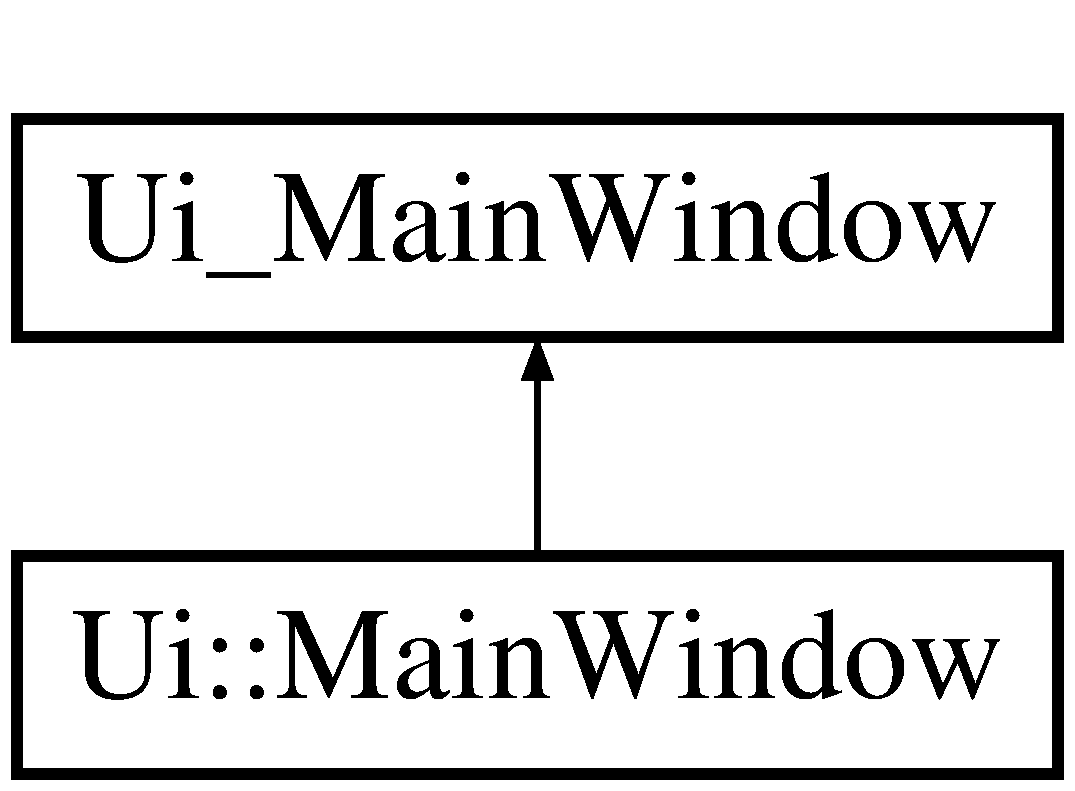
\includegraphics[height=2.000000cm]{class_ui___main_window}
\end{center}
\end{figure}
\subsection*{Public Member Functions}
\begin{DoxyCompactItemize}
\item 
\hypertarget{class_ui___main_window_acf4a0872c4c77d8f43a2ec66ed849b58}{void {\bfseries setup\-Ui} (Q\-Main\-Window $\ast$\hyperlink{class_main_window}{Main\-Window})}\label{class_ui___main_window_acf4a0872c4c77d8f43a2ec66ed849b58}

\item 
\hypertarget{class_ui___main_window_a097dd160c3534a204904cb374412c618}{void {\bfseries retranslate\-Ui} (Q\-Main\-Window $\ast$\hyperlink{class_main_window}{Main\-Window})}\label{class_ui___main_window_a097dd160c3534a204904cb374412c618}

\end{DoxyCompactItemize}
\subsection*{Public Attributes}
\begin{DoxyCompactItemize}
\item 
\hypertarget{class_ui___main_window_a30075506c2116c3ed4ff25e07ae75f81}{Q\-Widget $\ast$ {\bfseries central\-Widget}}\label{class_ui___main_window_a30075506c2116c3ed4ff25e07ae75f81}

\item 
\hypertarget{class_ui___main_window_a0c01bad60d9f422a1258e710635a2f65}{Q\-V\-Box\-Layout $\ast$ {\bfseries vertical\-Layout\-\_\-2}}\label{class_ui___main_window_a0c01bad60d9f422a1258e710635a2f65}

\item 
\hypertarget{class_ui___main_window_a8d440a6df1de0bc57afcdda7476d8f19}{Q\-Stacked\-Widget $\ast$ {\bfseries stacked\-Widget}}\label{class_ui___main_window_a8d440a6df1de0bc57afcdda7476d8f19}

\item 
\hypertarget{class_ui___main_window_ad7d164376bef8649ee1f94697b859417}{Q\-Widget $\ast$ {\bfseries page}}\label{class_ui___main_window_ad7d164376bef8649ee1f94697b859417}

\item 
\hypertarget{class_ui___main_window_a38b8a4b887f3b58e2a49e7905ae6f1f0}{Q\-V\-Box\-Layout $\ast$ {\bfseries vertical\-Layout\-\_\-3}}\label{class_ui___main_window_a38b8a4b887f3b58e2a49e7905ae6f1f0}

\item 
\hypertarget{class_ui___main_window_ac845bdf6b5b5237378a7b067808b7a31}{Q\-Spacer\-Item $\ast$ {\bfseries vertical\-Spacer\-\_\-3}}\label{class_ui___main_window_ac845bdf6b5b5237378a7b067808b7a31}

\item 
\hypertarget{class_ui___main_window_ad9c89133780f28e6efa2ec17ceb9cff5}{Q\-Label $\ast$ {\bfseries label}}\label{class_ui___main_window_ad9c89133780f28e6efa2ec17ceb9cff5}

\item 
\hypertarget{class_ui___main_window_adc1f5fdd97fb3729999c56902d0fa591}{Q\-Spacer\-Item $\ast$ {\bfseries vertical\-Spacer\-\_\-2}}\label{class_ui___main_window_adc1f5fdd97fb3729999c56902d0fa591}

\item 
\hypertarget{class_ui___main_window_acd6fdc9ebacc4b25b834162380d75ce8}{Q\-H\-Box\-Layout $\ast$ {\bfseries horizontal\-Layout}}\label{class_ui___main_window_acd6fdc9ebacc4b25b834162380d75ce8}

\item 
\hypertarget{class_ui___main_window_ad8088cf292df452936fc6d22aa40e1ab}{Q\-Push\-Button $\ast$ {\bfseries push\-Button\-Client}}\label{class_ui___main_window_ad8088cf292df452936fc6d22aa40e1ab}

\item 
\hypertarget{class_ui___main_window_a3ecc1465bdd3013fceb02aba167a5974}{Q\-Push\-Button $\ast$ {\bfseries push\-Button\-Serveur}}\label{class_ui___main_window_a3ecc1465bdd3013fceb02aba167a5974}

\item 
\hypertarget{class_ui___main_window_a09c2c2f371136ded0aa1f51b6d930d28}{Q\-Push\-Button $\ast$ {\bfseries push\-Button\-Solo}}\label{class_ui___main_window_a09c2c2f371136ded0aa1f51b6d930d28}

\item 
\hypertarget{class_ui___main_window_aa759396899fd5dce671f04d1b2fd3285}{Q\-Push\-Button $\ast$ {\bfseries push\-Button\-Solo\-Ia}}\label{class_ui___main_window_aa759396899fd5dce671f04d1b2fd3285}

\item 
\hypertarget{class_ui___main_window_a8384329c3663ff274e926a12024aab52}{Q\-Spacer\-Item $\ast$ {\bfseries vertical\-Spacer}}\label{class_ui___main_window_a8384329c3663ff274e926a12024aab52}

\item 
\hypertarget{class_ui___main_window_adcb6de4cebc6760fe319711f125010cc}{Q\-Widget $\ast$ {\bfseries page\-\_\-2}}\label{class_ui___main_window_adcb6de4cebc6760fe319711f125010cc}

\item 
\hypertarget{class_ui___main_window_a6f40fc110b15410c00837a446d57bdbe}{Q\-V\-Box\-Layout $\ast$ {\bfseries vertical\-Layout\-\_\-4}}\label{class_ui___main_window_a6f40fc110b15410c00837a446d57bdbe}

\item 
\hypertarget{class_ui___main_window_ab676f235c393f334b7c07935d4007925}{Q\-Widget $\ast$ {\bfseries widget}}\label{class_ui___main_window_ab676f235c393f334b7c07935d4007925}

\item 
\hypertarget{class_ui___main_window_a3b659bbe89dcd06d32a7039a432ff110}{Q\-Grid\-Layout $\ast$ {\bfseries grid\-Layout\-Jeu}}\label{class_ui___main_window_a3b659bbe89dcd06d32a7039a432ff110}

\item 
\hypertarget{class_ui___main_window_a17207206e55a605ecc14a3534b7e575f}{Q\-Frame $\ast$ {\bfseries line\-\_\-2}}\label{class_ui___main_window_a17207206e55a605ecc14a3534b7e575f}

\item 
\hypertarget{class_ui___main_window_aef7cb3be8cecfc9aaf98f036a98781ce}{Q\-Group\-Box $\ast$ {\bfseries group\-Box}}\label{class_ui___main_window_aef7cb3be8cecfc9aaf98f036a98781ce}

\item 
\hypertarget{class_ui___main_window_aecd96a04789fcfec3f98d80390ad8184}{Q\-V\-Box\-Layout $\ast$ {\bfseries vertical\-Layout}}\label{class_ui___main_window_aecd96a04789fcfec3f98d80390ad8184}

\item 
\hypertarget{class_ui___main_window_a80867018070156432923d0266cc9fe25}{Q\-H\-Box\-Layout $\ast$ {\bfseries horizontal\-Layout\-\_\-2}}\label{class_ui___main_window_a80867018070156432923d0266cc9fe25}

\item 
\hypertarget{class_ui___main_window_a26cbce0e8aa487ae7eab3bdee570350a}{Q\-Label $\ast$ {\bfseries label\-Joueur1}}\label{class_ui___main_window_a26cbce0e8aa487ae7eab3bdee570350a}

\item 
\hypertarget{class_ui___main_window_a8769023d1014e31b6afe4525ebb22a3f}{Q\-Label $\ast$ {\bfseries label\-Joueur2}}\label{class_ui___main_window_a8769023d1014e31b6afe4525ebb22a3f}

\item 
\hypertarget{class_ui___main_window_a9a43633211d56018140b0d718e9fcc2e}{Q\-H\-Box\-Layout $\ast$ {\bfseries horizontal\-Layout\-Joueurs}}\label{class_ui___main_window_a9a43633211d56018140b0d718e9fcc2e}

\item 
\hypertarget{class_ui___main_window_ae183387a7d233b437a637b403ba39ffd}{Q\-H\-Box\-Layout $\ast$ {\bfseries horizontal\-Layout\-\_\-4}}\label{class_ui___main_window_ae183387a7d233b437a637b403ba39ffd}

\item 
\hypertarget{class_ui___main_window_a5731ca480b84d22f9c8e94027e86e0c2}{Q\-Progress\-Bar $\ast$ {\bfseries progress\-Bar\-Tour}}\label{class_ui___main_window_a5731ca480b84d22f9c8e94027e86e0c2}

\item 
\hypertarget{class_ui___main_window_ad96a0a746b68d03e700e0bf4c899d389}{Q\-Push\-Button $\ast$ {\bfseries push\-Button\-Nouvelle\-Partie}}\label{class_ui___main_window_ad96a0a746b68d03e700e0bf4c899d389}

\item 
\hypertarget{class_ui___main_window_a27e0b134c3c12643afbf0b50dd175453}{Q\-Frame $\ast$ {\bfseries line\-\_\-3}}\label{class_ui___main_window_a27e0b134c3c12643afbf0b50dd175453}

\item 
\hypertarget{class_ui___main_window_ae54cc2b98c90284565a9dd3ce00ddb67}{Q\-Push\-Button $\ast$ {\bfseries push\-Button\-\_\-\-Quitter}}\label{class_ui___main_window_ae54cc2b98c90284565a9dd3ce00ddb67}

\item 
\hypertarget{class_ui___main_window_ac682cb2a9b686ca7c3d29771ad9ccb48}{Q\-Widget $\ast$ {\bfseries page\-\_\-3}}\label{class_ui___main_window_ac682cb2a9b686ca7c3d29771ad9ccb48}

\item 
\hypertarget{class_ui___main_window_afcc20a3d5058037a00cdc6122f231848}{Q\-V\-Box\-Layout $\ast$ {\bfseries vertical\-Layout\-\_\-5}}\label{class_ui___main_window_afcc20a3d5058037a00cdc6122f231848}

\item 
\hypertarget{class_ui___main_window_a2e2516d755e4dd53fc905dabddf2738a}{Q\-Label $\ast$ {\bfseries label\-\_\-2}}\label{class_ui___main_window_a2e2516d755e4dd53fc905dabddf2738a}

\item 
\hypertarget{class_ui___main_window_af984dda6e986374c3b4e1f5d1e3704d1}{Q\-Push\-Button $\ast$ {\bfseries push\-Button\-Annuler\-La\-Recherche}}\label{class_ui___main_window_af984dda6e986374c3b4e1f5d1e3704d1}

\end{DoxyCompactItemize}


The documentation for this class was generated from the following file\-:\begin{DoxyCompactItemize}
\item 
ui\-\_\-mainwindow.\-h\end{DoxyCompactItemize}

%--- End generated contents ---

% Index
\newpage
\phantomsection
\addcontentsline{toc}{part}{Index}
\printindex

\end{document}
